\chapter{Memory Management}\label{chapter:Memory Management}

The objective here is to support \textbf{malloc()} and \textbf{free()}.
The implementation of memory management is split into two phases:
\begin{itemize}
    \item Implementing Physical Memory allocator
    \item Porting liballoc
\end{itemize}

\section{Physical Memory Allocator}\label{section:Physical Memory Allocator}

This idea here is to allocate memory in 4kb chunks. Liballoc will use this allocator internally to provide malloc()
functionality. A simplified overview of the implementation is as follows:
\begin{enumerate}
    \item Split physical memory into blocks of size 4kb each.
    \item Use a data structure to keep track of which regions are free/used.
    \item Provide an API to allocate/free blocks.
\end{enumerate} 
These steps are elaborated in the following subsections.
\pagebreak

\subsection{Memory Map}\label{subsection:Memory Map}
A memory map is a data structure that gives indication about the status of different regions of physical memory.
DaxOS uses multiboot to fetch the memory map. \\

The following multiboot struct represents information about a single memory\\ region:
\begin{lstlisting}
    typedef struct multiboot_memory_map {
        uint32_t size;
        uint32_t base_addr_low, base_addr_high;
        uint32_t length_low, length_high;
        uint32_t type;
    };
\end{lstlisting}
\begin{itemize}
    \item \textbf{size}: Size of this structure. 
    \item \textbf{base\_addr\_low, base\_addr\_high}: Starting address of this memory region.
    \item \textbf{length\_low, length\_high}: Length of this memory region in bytes.
    \item \textbf{type}: Status of this region. A value of `1' here indicates available.
\end{itemize}

We can configure multiboot to pass this information to our kernel by modifying \textbf{boot.S} as follows:
\vspace{0.5cm}
\begin{lstlisting}
    .set MEMINFO,  1<<1   # provide memory map
    .set FLAGS,    ALIGN | MEMINFO
\end{lstlisting}
\vspace{0.5cm}

We can get the information of the next region by adding \textit{size} bytes to the memory address of this record.

\begin{figure}[h!]
	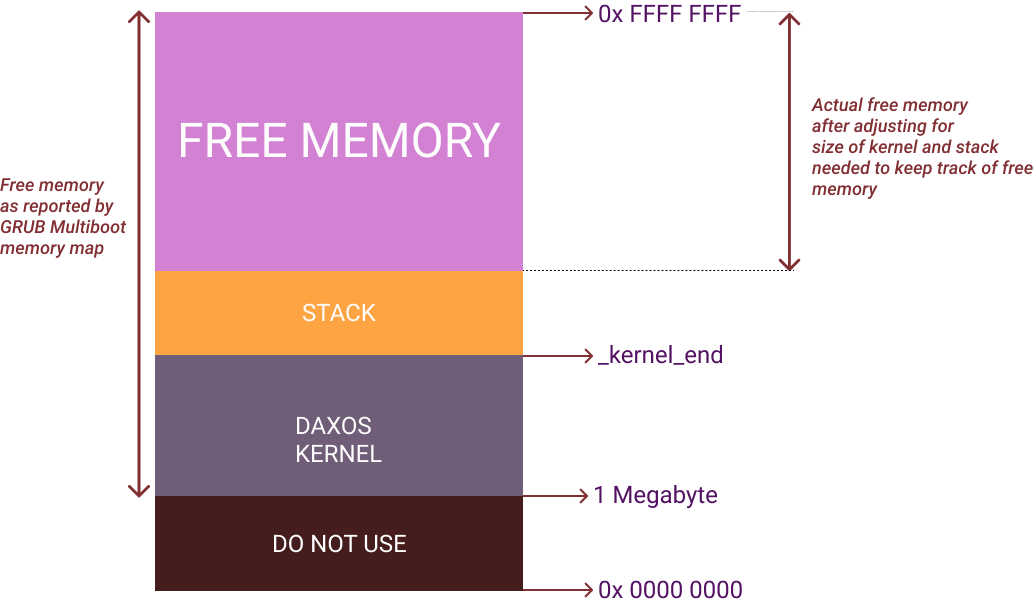
\includegraphics[width=\textwidth,height=\textheight,keepaspectratio]{mem_arch}
	\caption{Memory Architecture in DaxOS}
\end{figure}
\clearpage

\pagebreak
\subsection{Keeping Track of Memory}\label{subsection:Keeping Track of Memory}

With the memory map in possession, the next objective is to implement a data structure to keep track of this memory.
There are two common options:
\begin{itemize}
    \item \textbf{Bitmap}
    \item \textbf{Stack}
\end{itemize}

The disadvantage of using a bitmap is that in order to find a free 4kb block of memory, the entire data structure needs
to be scanned. This incurs a run-time complexity of O(n).
Using a stack is O(1) since all that is required to find a free block is simply a pop operation.
Therefore DaxOS uses the stack approach.

\vspace{1cm}
The stack implementation supports two calls:
\begin{lstlisting}
    void push(uint32_t mem_addr);
    int32_t pop();
\end{lstlisting}

\subsection{API}\label{subsection:API}
The API consists of two calls:
\vspace{0.3cm}
\begin{lstlisting}
    uint32_t* get_page();
    void free_page(uint32_t *page);
\end{lstlisting}
Their description is as follows:
\begin{itemize}
    \item \textbf{get\_page()}: returns the memory address of a free 4kb block of memory.
    \item \textbf{free\_page()}: returns the block to the free list.
\end{itemize}
\pagebreak

\section{Porting Liballoc}\label{section:Porting liballoc}

Liballoc is a free and open-source memory allocator for use in hobbyist OS. 
It provides malloc and other related functions. However to use liballoc, DaxOS must implement four hooks.
Hooks are functions that liballoc uses internally that must be provided by the OS.

\vspace{0.3cm}
The hooks are:
\begin{lstlisting}
    extern int liballoc_lock();
    extern int liballoc_unlock();
    extern void *liballoc_alloc(size_t);
    extern int liballoc_free(void *, size_t);
\end{lstlisting}

Their descriptions are as follows:
\begin{itemize}
    \item \textbf{Lock and unlock} are used to provide mutex locks.\\
    Although DaxOS is not multi-threaded it still has concurrency in the form of interrupts.
    Therefore the lock function simply disables interrupts whereas the unlock function enables interrupts.
    This is done using the \textit{cli} and \textit{sti} instructions respectively.
    \item \textbf{alloc} function allocates multiple blocks of memory as specified in the parameter.
    \item \textbf{free} function frees multiple blocks of memory starting from the address specified in parameter.
\end{itemize}

These functions are implemented using the functions in the physical memory allocator.
At this point, implementation of memory management is complete.
